%% latex command to generate:
%% pdflatex -shell-escape figures
\documentclass[journal]{IEEEtranTIE}
\usepackage{graphicx}
\usepackage[noadjust]{cite}
\usepackage{picinpar}
\usepackage{amsmath}
\usepackage{stfloats}
%%\usepackage{dblfloatfix}
\usepackage{url}
\usepackage{flushend}
\usepackage[latin1]{inputenc}
\usepackage{colortbl}
\usepackage{soul}
\usepackage{multirow}
\usepackage{pifont}
\usepackage{color}
\usepackage{alltt}
\usepackage[hidelinks]{hyperref}
\usepackage{enumerate}
\usepackage{siunitx}
\usepackage{breakurl}
\usepackage{epstopdf}
\usepackage{pbox}

%% My packages
%% \usepackage[cmex10]{amsmath}
%% \interdisplaylinepenalty=2500
\usepackage{algpseudocode}
%% \usepackage{array}
\usepackage[caption=false,font=footnotesize]{subfig}

\usepackage{tikz}
\usetikzlibrary{external}
\usetikzlibrary{arrows.meta}
\tikzexternalize[prefix=./] %  activate
%% \usepackage{mathabx}


\newcommand{\hide}[1]{\ignorespaces}
\newcommand{\jx}[1]{{\bf Jiaxiang: }#1{ \bf End}}
\newtheorem{theorem}{Theorem}
\newtheorem{lemma}[theorem]{Lemma}
\newtheorem{definition}[theorem]{Definition}

% Define the fontsize in environment {verbatim}
\makeatletter
\def\verbatim{\small\@verbatim \frenchspacing\@vobeyspaces \@xverbatim}
\makeatother

\usepackage{microtype}

\begin{document}

\tikzsetnextfilename{FIG2_15-TIE-3480}
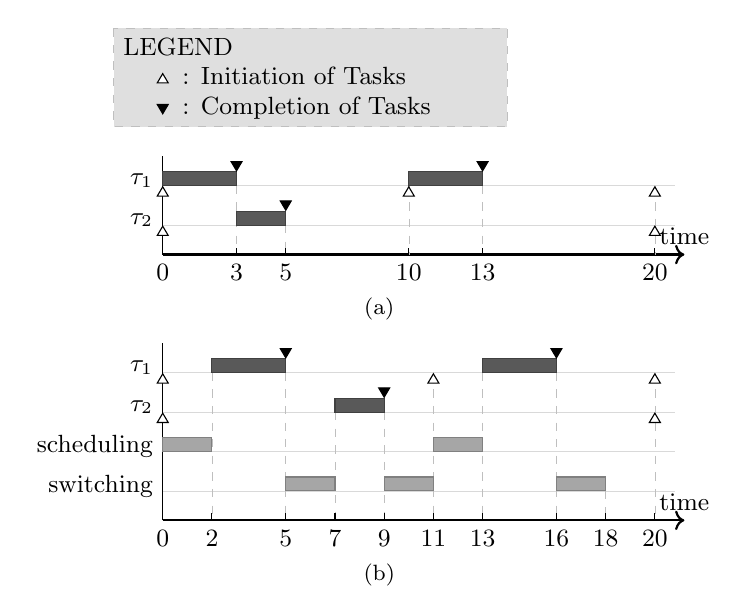
\begin{tikzpicture}[font=\small,scale=1.25,
    % styles
    system task/.style={fill=gray!70,draw=gray},
    periodic task/.style={fill=gray!70!black,draw=gray!50!black},
    task line/.style={gray!30,very thin},
    time line/.style={gray!50,very thin,dashed},
    short line/.style={gray!50,very thin,dashed},
    init/.style={{Triangle[fill=white,scale=1.1]}-},
    complete/.style={{Triangle[scale=1.1]}-}]

  % legend
  \begin{scope}[xshift=-2cm]  
    \draw [fill=gray!25,draw=gray!50,dashed] (1.5,2.3) rectangle +(4,-1);
    \draw (1.5,2.3) node [below right] {LEGEND};
    \draw [init] (2,1.85) -- +(0,-0.01);
    \draw (2.1,2) node [below right] {: Initiation of Tasks};
    \draw [complete] (2,1.42) -- +(0,0.1);
    \draw (2.1,1.7) node [below right] {: Completion of Tasks};
  \end{scope}

  %%% RMS Algorithm
  \begin{scope}
  
    % grid
    \foreach \x in {0.3,0.7}
      \draw[task line] (0,\x) -- (5.2,\x);

    % axes
    \draw[->,thick] (0,0) node [below] {$0$} -- (5.3,0) node [above] {time};
    \draw[thin] (0,0) -- (0,1);

    % time indicator
    \draw [time line] (0.75,0.7) -- (0.75,0);
    \draw (0.75,0) node [below] {$3$} -- +(0,2pt);
    \draw [time line] (1.25,0.3) -- (1.25,0);
    \draw (1.25,0) node [below] {$5$} -- +(0,2pt);
    \draw [time line] (2.5,0.7) -- (2.5,0);
    \draw (2.5,0) node [below] {$10$} -- +(0,2pt);
    \draw [time line] (3.25,0.7) -- (3.25,0);
    \draw (3.25,0) node [below] {$13$} -- +(0,2pt);

    \draw [time line] (5,0.7) -- (5,0);
    \draw (5,0) node [below] {$20$} -- +(0,2pt);
    
    % tasks
    \draw [periodic task] (0,0.7) rectangle +(0.75,0.14);
    \draw [periodic task] (0.75,0.3) rectangle +(0.5,0.14);
    \draw [periodic task] (2.5,0.7) rectangle +(0.75,0.14);

    % text
    \draw (0,0.75) node [left] {$\tau_1$};
    \draw (0,0.35) node [left] {$\tau_2$};
    \path (0,0.75) node [left,text opacity=0] {scheduling};
    \path (0,0.35) node [left,text opacity=0] {switching};    

    % initiation of tasks
    \foreach \x in {0,2.5,5}
      \draw [init] (\x,0.7) -- +(0,-0.01);
    \foreach \x in {0,5}
      \draw [init] (\x,0.3) -- +(0,-0.01);  

    % completion of tasks
    \draw [complete] (0.75,0.84) -- +(0,0.01);
    \draw [complete] (3.25,0.84) -- +(0,0.01);
    \draw [complete] (1.25,0.44) -- +(0,0.01);

    % label of subfigure
    \draw (2.2,-0.55) node [inner sep=0pt] {\footnotesize (a)};

  \end{scope}

  %%% RMS Implementation
  \begin{scope}[yshift=-2.7cm]

    % grid
    \foreach \x in {0.3,0.7,1.1,1.5}
      \draw[task line] (0,\x) -- (5.2,\x);

    % axes
    \draw[->,thick] (0,0) node [below] {$0$} -- (5.3,0) node [above] {time};
    \draw[thin] (0,0) -- (0,1.8);

    % time indicator
    \draw [time line] (0.5,1.5) -- (0.5,0);
    \draw (0.5,0) node [below] {$2$} -- +(0,2pt);
    \draw [time line] (1.25,1.5) -- (1.25,0);
    \draw (1.25,0) node [below] {$5$} -- +(0,2pt);
    \draw [time line] (1.75,1.1) -- (1.75,0);
    \draw (1.75,0) node [below] {$7$} -- +(0,2pt);
    \draw [time line] (2.25,1.1) -- (2.25,0);
    \draw (2.25,0) node [below] {$9$} -- +(0,2pt);
    \draw [time line] (2.75,1.5) -- (2.75,0);
    \draw (2.75,0) node [below] {$11$} -- +(0,2pt);
    \draw [time line] (3.25,1.5) -- (3.25,0);
    \draw (3.25,0) node [below] {$13$} -- +(0,2pt);
    \draw [time line] (4,1.5) -- (4,0);
    \draw (4,0) node [below] {$16$} -- +(0,2pt);
    \draw [time line] (4.5,0.3) -- (4.5,0);
    \draw (4.5,0) -- +(0,2pt);
    \draw (4.5,0) node [below] {$18$};
    \draw [time line] (5,1.5) -- (5,0);
    \draw (5,0) node [below] {$20$} -- +(0,2pt);
    
    % tasks
    \draw [system task] (0,0.7) rectangle +(0.5,0.14);
    \draw [periodic task] (0.5,1.5) rectangle +(0.75,0.14);
    \draw [system task] (1.25,0.3) rectangle +(0.5,0.14);
    \draw [periodic task] (1.75,1.1) rectangle +(0.5,0.14);
    \draw [system task] (2.25,0.3) rectangle +(0.5,0.14);
    \draw [system task] (2.75,0.7) rectangle +(0.5,0.14);
    \draw [periodic task] (3.25,1.5) rectangle +(0.75,0.14);
    \draw [system task] (4,0.3) rectangle +(0.5,0.14);

    % text
    \draw (0,1.55) node [left] {$\tau_1$};
    \draw (0,1.15) node [left] {$\tau_2$};
    \draw (0,0.75) node [left] {scheduling};
    \draw (0,0.35) node [left] {switching};    

    % initiation of tasks
    \foreach \x in {0,2.75,5}
      \draw [init] (\x,1.5) -- +(0,-0.01);
    \foreach \x in {0,5}
      \draw [init] (\x,1.1) -- +(0,-0.01);  

    % completion of tasks
    \draw [complete] (1.25,1.64) -- +(0,0.01);
    \draw [complete] (2.25,1.24) -- +(0,0.01);
    \draw [complete] (4,1.64) -- +(0,0.01);
    
    % label of subfigure
    \draw (2.2,-0.55) node [inner sep=0pt] {\footnotesize (b)};
  \end{scope}
\end{tikzpicture}

\tikzsetnextfilename{FIG3_15-TIE-3480}
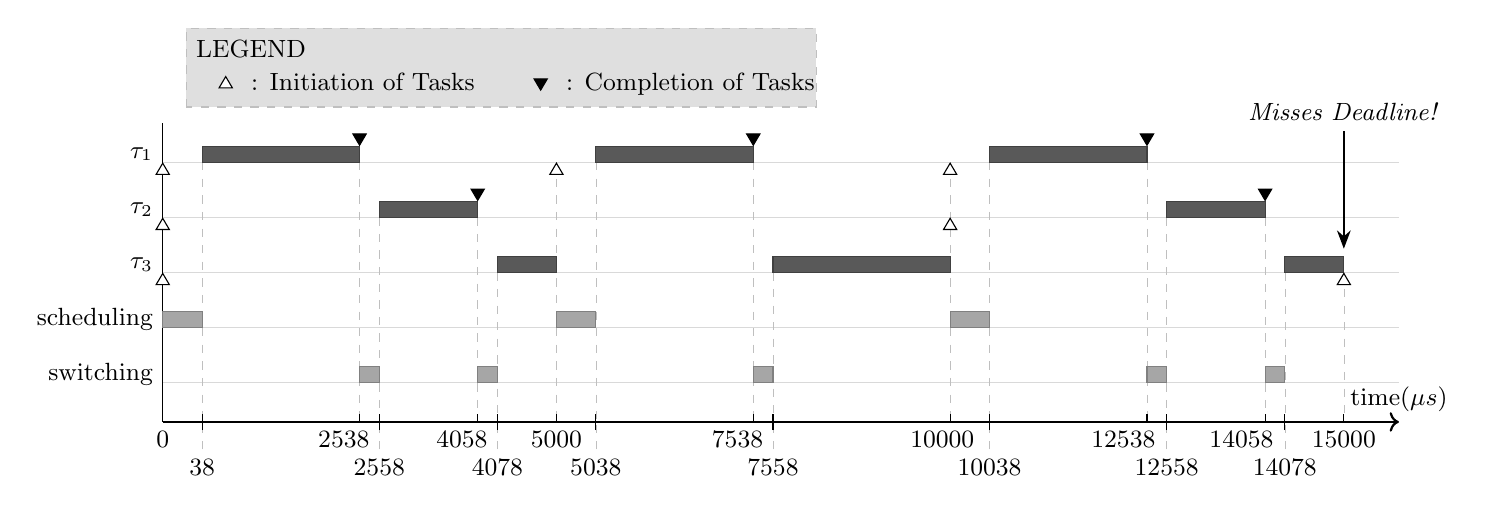
\begin{tikzpicture}[font=\small,
    % styles
    system task/.style={fill=gray!70,draw=gray},
    periodic task/.style={fill=gray!70!black,draw=gray!50!black},
    task line/.style={gray!30,very thin},
    time line/.style={gray!50,very thin,dashed},
    short line/.style={gray!50,very thin,dashed},
    init/.style={{Triangle[fill=white,scale=1.3]}-},
    complete/.style={{Triangle[scale=1.3]}-}]

  % grid
  \foreach \x in {0.5,1.2,...,3.3}
    \draw[task line] (0,\x) -- (15.7,\x);

  % time indicator
  \draw (0,0) node [below] {$0$};
  \draw[time line] (0.5,3.3) -- (0.5,0);
  \draw (0.5,-0.35) node [below] {$38$} [short line] -- +(0,0.35);
  \draw (0.5,-3pt) -- (0.5,3pt);
  \draw[time line] (2.5,3.3) -- (2.5,0);
  \draw (2.3,0) node [below] {$2538$};
  \draw (2.5,0) -- (2.5,3pt);
  \draw[time line] (2.75,2.6) -- (2.75,0);
  \draw (2.75,-0.35) node [below] {$2558$} [short line] -- +(0,0.35);
  \draw (2.75,-3pt) -- (2.75,3pt);
  \draw[time line] (4,2.6) -- (4,0);
  \draw (3.8,0) node [below] {$4058$};
  \draw (4,0) -- (4,3pt);
  \draw[time line] (4.25,1.9) -- (4.25,0);
  \draw (4.25,-0.35) node [below] {$4078$} [short line] -- +(0,0.35);
  \draw (4.25,-3pt) -- (4.25,3pt);

  \draw[time line] (5,3.3) -- (5,0);
  \draw (5,0) node [below] {$5000$};
  \draw (5,0) -- (5,3pt);
  \draw[time line] (5.5,3.3) -- (5.5,0);
  \draw (5.5,-0.35) node [below] {$5038$} [short line] -- +(0,0.35);
  \draw (5.5,-3pt) -- (5.5,3pt);
  \draw[time line] (7.5,3.3) -- (7.5,0);
  \draw (7.3,0) node [below] {$7538$};
  \draw (7.5,0) -- (7.5,3pt);
  \draw[time line] (7.75,1.9) -- (7.75,0);
  \draw (7.75,-0.35) node [below] {$7558$} [short line] -- +(0,0.35);
  \draw (7.75,-3pt) -- (7.75,3pt);

  \draw[time line] (10,3.3) -- (10,0);
  \draw (9.9,0) node [below] {$10000$};
  \draw (10,0) -- (10,3pt);
  \draw[time line] (10.5,3.3) -- (10.5,0);
  \draw (10.5,-0.35) node [below] {$10038$} [short line] -- +(0,0.35);
  \draw (10.5,-3pt) -- (10.5,3pt);
  \draw[time line] (12.5,3.3) -- (12.5,0);
  \draw (12.2,0) node [below] {$12538$};
  \draw (12.5,0) -- (12.5,3pt);
  \draw[time line] (12.75,2.6) -- (12.75,0);
  \draw (12.75,-0.35) node [below] {$12558$} [short line] -- +(0,0.35);
  \draw (12.75,-3pt) -- (12.75,3pt);
  \draw[time line] (14,2.6) -- (14,0);
  \draw (13.7,0) node [below] {$14058$};
  \draw (14,0) -- (14,3pt);
  \draw[time line] (14.25,1.9) -- (14.25,0);
  \draw (14.25,-0.35) node [below] {$14078$} [short line] -- +(0,0.35);
  \draw (14.25,-3pt) -- (14.25,3pt);
  \draw[time line] (15,1.9) -- (15,0);
  \draw (15,0) node [below] {$15000$};
  \draw (15,0) -- (15,3pt);

  % axes
  \draw[->,thick] (0,0) -- (15.7,0) node [above] {time(${\mu}s$)};
  \draw[thin] (0,0) -- (0,3.8);

  % tips of tasks
  \draw (0,0.6) node [left] {switching};
  \draw (0,1.3) node [left] {scheduling};
  \draw (0,2) node [left] {$\tau_3$};
  \draw (0,2.7) node [left] {$\tau_2$};
  \draw (0,3.4) node [left] {$\tau_1$};

  % tasks
  \filldraw[system task] (0,1.2) rectangle +(0.5,0.2);
  \filldraw[periodic task] (0.5,3.3) rectangle +(2,0.2);
  \filldraw[system task] (2.5,0.5) rectangle +(0.25,0.2);
  \filldraw[periodic task] (2.75,2.6) rectangle +(1.25,0.2);
  \filldraw[system task] (4,0.5) rectangle +(0.25,0.2);
  \filldraw[periodic task] (4.25,1.9) rectangle +(0.75,0.2);
  
  \filldraw[system task] (5,1.2) rectangle +(0.5,0.2);
  \filldraw[periodic task] (5.5,3.3) rectangle +(2,0.2);
  \filldraw[system task] (7.5,0.5) rectangle +(0.25,0.2);
  \filldraw[periodic task] (7.75,1.9) rectangle +(2.25,0.2);
  
  \filldraw[system task] (10,1.2) rectangle +(0.5,0.2);
  \filldraw[periodic task] (10.5,3.3) rectangle +(2,0.2);
  \filldraw[system task] (12.5,0.5) rectangle +(0.25,0.2);
  \filldraw[periodic task] (12.75,2.6) rectangle +(1.25,0.2);
  \filldraw[system task] (14,0.5) rectangle +(0.25,0.2);
  \filldraw[periodic task] (14.25,1.9) rectangle +(0.75,0.2);

  % initiation of tasks
  \foreach \x in {0,5,10}
    \draw [init] (\x,3.3) -- +(0,-0.1);
  \foreach \x in {0,10}
    \draw [init] (\x,2.6) -- +(0,-0.1);  
  \foreach \x in {0,15}
    \draw [init] (\x,1.9) -- +(0,-0.1); 

  % completion of tasks
  \draw [complete] (2.5,3.5) -- +(0,0.1);
  \draw [complete] (4,2.8) -- +(0,0.1);
  \draw [complete] (7.5,3.5) -- +(0,0.1);
  \draw [complete] (12.5,3.5) -- +(0,0.1);
  \draw [complete] (14,2.8) -- +(0,0.1);

  % text
  \draw[{Stealth}-,thick] (15,2.2) -- +(0,1.5)
    node [above] {\emph{Misses Deadline!}};

  % legend
  \begin{scope}[xshift = -1.2cm]  
    \draw [fill=gray!25,draw=gray!50,dashed] (1.5,4) rectangle +(8,1);
    \draw (1.5,4.5) node [above right] {LEGEND};
    \draw [init] (2,4.4) -- +(0,-0.1);
    \draw (2.2,4.55) node [below right] {: Initiation of Tasks};
    \draw [complete] (6,4.2) -- +(0,0.1);
    \draw (6.2,4.55) node [below right] {: Completion of Tasks};
  \end{scope}
\end{tikzpicture}
\end{document}
